\documentclass[12pt, spanish]{article}
\newcommand\tab[1][1cm]{\hspace*{#1}}
\usepackage[spanish]{babel}
\selectlanguage{spanish}
\usepackage{natbib}
\usepackage{url}
\usepackage[utf8x]{inputenc}
\usepackage{graphicx}
\graphicspath{{images/}}
\usepackage{parskip}
\usepackage{fancyhdr}
\usepackage{vmargin}
\usepackage{multirow}
\usepackage{pgfplots}
\usepackage{float}
\usepackage{algorithm}
\usepackage{algorithmic}
\usepackage{chngpage}
\usepackage{enumitem}
\usepackage{amsmath}
\usepackage{algorithm}
\usepackage{algpseudocode}

\usepackage{subcaption}

\usepackage{hyperref}
\usepackage[
    type={CC},
    modifier={by-nc-sa},
    version={4.0},
]{doclicense}

\hypersetup{
    colorlinks=true,
    linkcolor=blue,
    filecolor=magenta,      
    urlcolor=cyan,
}

% para codigo
\usepackage{listings}
\usepackage{xcolor}



%% configuración de listings

\definecolor{listing-background}{HTML}{F7F7F7}
\definecolor{listing-rule}{HTML}{B3B2B3}
\definecolor{listing-numbers}{HTML}{B3B2B3}
\definecolor{listing-text-color}{HTML}{000000}
\definecolor{listing-keyword}{HTML}{435489}
\definecolor{listing-identifier}{HTML}{435489}
\definecolor{listing-string}{HTML}{00999A}
\definecolor{listing-comment}{HTML}{8E8E8E}
\definecolor{listing-javadoc-comment}{HTML}{006CA9}

\lstdefinestyle{eisvogel_listing_style}{
  language         = c++,
%$if(listings-disable-line-numbers)$
%  xleftmargin      = 0.6em,
%  framexleftmargin = 0.4em,
%$else$
  numbers          = left,
  xleftmargin      = 0em,
 framexleftmargin = 0em,
%$endif$
  backgroundcolor  = \color{listing-background},
  basicstyle       = \color{listing-text-color}\small\ttfamily{}\linespread{1.15}, % print whole listing small
  breaklines       = true,
  frame            = single,
  framesep         = 0.19em,
  rulecolor        = \color{listing-rule},
  frameround       = ffff,
  tabsize          = 4,
  numberstyle      = \color{listing-numbers},
  aboveskip        = 1.0em,
  belowskip        = 0.1em,
  abovecaptionskip = 0em,
  belowcaptionskip = 1.0em,
  keywordstyle     = \color{listing-keyword}\bfseries,
  classoffset      = 0,
  sensitive        = true,
  identifierstyle  = \color{listing-identifier},
  commentstyle     = \color{listing-comment},
  morecomment      = [s][\color{listing-javadoc-comment}]{/**}{*/},
  stringstyle      = \color{listing-string},
  showstringspaces = false,
  escapeinside     = {/*@}{@*/}, % Allow LaTeX inside these special comments
  literate         =
  {á}{{\'a}}1 {é}{{\'e}}1 {í}{{\'i}}1 {ó}{{\'o}}1 {ú}{{\'u}}1
  {Á}{{\'A}}1 {É}{{\'E}}1 {Í}{{\'I}}1 {Ó}{{\'O}}1 {Ú}{{\'U}}1
  {à}{{\`a}}1 {è}{{\'e}}1 {ì}{{\`i}}1 {ò}{{\`o}}1 {ù}{{\`u}}1
  {À}{{\`A}}1 {È}{{\'E}}1 {Ì}{{\`I}}1 {Ò}{{\`O}}1 {Ù}{{\`U}}1
  {ä}{{\"a}}1 {ë}{{\"e}}1 {ï}{{\"i}}1 {ö}{{\"o}}1 {ü}{{\"u}}1
  {Ä}{{\"A}}1 {Ë}{{\"E}}1 {Ï}{{\"I}}1 {Ö}{{\"O}}1 {Ü}{{\"U}}1
  {â}{{\^a}}1 {ê}{{\^e}}1 {î}{{\^i}}1 {ô}{{\^o}}1 {û}{{\^u}}1
  {Â}{{\^A}}1 {Ê}{{\^E}}1 {Î}{{\^I}}1 {Ô}{{\^O}}1 {Û}{{\^U}}1
  {œ}{{\oe}}1 {Œ}{{\OE}}1 {æ}{{\ae}}1 {Æ}{{\AE}}1 {ß}{{\ss}}1
  {ç}{{\c c}}1 {Ç}{{\c C}}1 {ø}{{\o}}1 {å}{{\r a}}1 {Å}{{\r A}}1
  {€}{{\EUR}}1 {£}{{\pounds}}1 {«}{{\guillemotleft}}1
  {»}{{\guillemotright}}1 {ñ}{{\~n}}1 {Ñ}{{\~N}}1 {¿}{{?`}}1
  {…}{{\ldots}}1 {≥}{{>=}}1 {≤}{{<=}}1 {„}{{\glqq}}1 {“}{{\grqq}}1
  {”}{{''}}1
}
\lstset{style=eisvogel_listing_style}


\usepackage[default]{sourcesanspro}

\setmarginsrb{2 cm}{1 cm}{2 cm}{2 cm}{1 cm}{1.5 cm}{1 cm}{1.5 cm}

\title{Práctica 3:\\
APC - Búsquedas por Trayectorias  \hspace{0.05cm} }                           
\author{Cristina Sánchez Justicia}                             
\date{\today}                                           

\renewcommand*\contentsname{hola}

\makeatletter
\let\thetitle\@title
\let\theauthor\@author
\let\thedate\@date
\makeatother

\pagestyle{fancy}
\fancyhf{}
\rhead{\theauthor}
\lhead{\thetitle}
\cfoot{\thepage}

\begin{document}

%%%%%%%%%%%%%%%%%%%%%%%%%%%%%%%%%%%%%%%%%%%%%%%%%%%%%%%%%%%%%%%%%%%%%%%%%%%%%%%%%%%%%%%%%

\begin{titlepage}
    \centering
    \vspace*{0.3 cm}
    
\includegraphics[scale = 0.50]{ugr.png}\\[0.7 cm]
    %\textsc{\LARGE Universidad de Granada}\\[2.0 cm]   
    \textsc{\large 3º CSI 2022/23 - Grupo 1}\\[0.5 cm]                \textsc{\large Grado en Ingeniería Informática}\\[0.5 cm]              
    \rule{\linewidth}{0.2 mm} \\[0.2 cm]
    { \huge \bfseries \thetitle}\\
	Algoritmos: 
	1-NN, RELIEF, BL, AGE-BLX, AGE-CA, BMB, ES, ILS, ILS-ES, VNS \\
    \rule{\linewidth}{0.2 mm} \\[1 cm]
    
    \begin{minipage}{0.4\textwidth}
        \begin{flushleft} \large
            \emph{Autor:}\\
            \theauthor\\ 
			 \emph{DNI:}\\
            77689772G
            \end{flushleft}
            \end{minipage}~
            \begin{minipage}{0.4\textwidth}
            \begin{flushright} \large
            \emph{Asignatura: \\
            Metaheurísticas}   \\     
            \emph{Correo:}\\
            cristina@correo.ugr.es           
        \end{flushright}
    \end{minipage}\\[0.5cm]
  
    {\large \thedate}\\[0.5cm]
    {\url{https://github.com/cristinasj/MH/}}
 	
    \vfill
    
\end{titlepage}

%%%%%%%%%%%%%%%%%%%%%%%%%%%%%%%%%%%%%%%%%%%%%%%%%%%%%%%%%%%%%%%%%%%%%%%%%%%%%%%%%%%%%%%%%

\tableofcontents
\pagebreak

%%%%%%%%%%%%%%%%%%%%%%%%%%%%%%%%%%%%%%%%%%%%%%%%%%%%%%%%%%%%%%%%%%%%%%%%%%%%%%%%%%%%%%%%%


\section{Descripción del problema}
Los problemas de clasificación son un clásico de la Inteligencia Artificial y, más específicamente, el Aprendizaje Automático. Los elementos con los que se trabajan en un problema de clasificación son un conjunto de datos, que pueden ser imágenes, audios, textos… Los cuales son fáciles de distinguir por un humano. Por ejemplo, un humano podría distinguir entre una imagen de un árbol y una imagen de una flor. El objetivo es conseguir de cualquier forma que un ordenador pueda clasificar de la misma forma, si no mejor, que un humano.  \\ \\
El Aprendizaje de Pesos en Características es una variación del problema de
clasificación en el que en nuestro conjunto de datos, por cada elemento tenemos un 
vector de características que lo definen. Este problema se puede solucionar de muchas 
maneras pero en esta práctica nosotros utilizaremos el claisificador K-NN, la Busqueda
Local, el método RELIEF, algoritmos genéticos estacionarios, Enfriamiento Simulado, 
Iterative Local Search, Busqueda Multiarranque Básica.  
\pagebreak

\section{Descripción de la aplicación de los algoritmos aplicados al problema }

Las consideraciones comunes a los distintos algoritmos son las siguientes: 

\subsection{Esquemas de representación}
Al igual que en anteriores prácticas la representación adoptada implica el uso de un vector W de longitud n, donde cada elemento tiene un valor en el rango [0, 1]. Este vector representa el peso asociado a cada característica y determina su capacidad para ser eliminada si su peso es menor que 0.1. \\
\newline 
Para representar esto se utilizan las siguientes estructuras de datos: 
\begin{enumerate}[label=-]
  \item Elemento: en la anterior práctica se utilizó una clase llamada Elemento. En esta práctica los elementos van en una matriz junto con una lista de caracteristicas paralela para ahorrar tiempo de ejecución.
  \item Set de datos: matriz bidimensional numpy donde cada fila representa un vector de caracteristicas y cada columna los valores de una caracteristica 
  \item  Soluciones: arrays de pesos paralelos a los vectores de características de cada elemento. Cada valor del array representa la importancia de cada característica para buscar la distancia mínima ponderada al utilizar el clasificador 1-NN. Sus valores están siempre entre 0 y 1. 
\end{enumerate}
\subsection{Descripción de la función objetivo }
La función objetivo se llama funciónEvaluacion y se dedica a dar una valoración numérica a unos pesos entrenados con los diferentes algoritmos. Para ello tiene en cuenta el porcentaje de reducción y el porcentaje de clasificación. En nuestro caso damos un 80\% de importancia a la clasificación y un 20\% de importancia a la reducción. \\
\newline
El porcentaje de reducción nos dice cómo de mucho se simplifica el problema con esos pesos. Es decir, a cuanto mayor sea el porcentaje de reducción, menos poder computacional es necesario para generar el resultado de clasificación al utilizar nuestro clasificador en producción, es decir, en un caso real. Este porcentaje de reducción se obtiene calculando el porcentaje de pesos que son cercanos a 0, es decir, el porcentaje de pesos que apenas importan información a la hora de clasificar a un individuo. \\
\newline
El porcentaje de clasificación nos dice el porcentaje de aciertos de nuestro clasificador. Para eso utiliza un conjunto de evaluación y un conjunto de entrenamiento y se ejecuta el clasificador 1-NN sobre cada elemento del conjunto de evaluación y respecto al conjunto de entrenamiento, usando una distancia ponderada dada por los pesos. 

\subsection{Descripción de los operadores comunes}
El operador distancia nos da la distancia cuadrada, euclídea y ponderada de un elemento a otro. La distancia es cuadada para ahorrar calculos y acelerar el proceso ya que no nos interesa el valor real en el cálculo de 1NN. La distancia es euclídea porque todas las variables en esta práctica son continuas. 
El operador distancia está implementado de la siguiente forma: 

function distancia (array\_caracteristicas uno, array\_caracteristicas otro, array\_caracteristicas pesos): \\ 
\tab    if pesos.esNulo( ):\\ 
\tab\tab 	    pesos.llenarDeUnos( )\\
devolver sumatoria((uno-otro)² * pesos)\\

\subsection{Pseudocódigo del proceso de generación de soluciones aleatorias}
La solución inicial se obtendrá de manera aleatoria en todos los casos, utilizando una distribución uniforme en el rango de [0, 1].\\
\newline
Para implementar esto, se utiliza la función rand de la biblioteca numpy y el módulo random como se muestra en este pseudocódigo:\\
\\
para\_cada i en (0, 1, 2, ...,  t\_poblacion):\\
\tab       	pesos = np.random.rand(datos.tamaño())\\
   \tab    	evaluacion = evaluar(datos, pesos) \\
\tab	poblacion.incluir(pesos, evaluacion)\\
end\_para\\

\subsection{Operador de cruce BLX}
Recibe dos cromosomas y genera dos descendientes generados aleatoriamente en un intervalo que depende de los valores de los padres. El pseudocódigo es el siguiente: \\
\\
funcion cruce\_BLX(cromosoma c1 ,cromosoma c2) devuelve una pareja de cromosomas:\\
\tab    para\_cada gen1 y gen2 en c1 y c2 :	\\
\tab\tab	alfa = 0.3\\
\tab\tab	min, max = devolverMinMax(gen1, gen2)\\
\tab\tab    	l = max-min\\
\tab\tab   	b1 = min-l*alfa\\
\tab\tab    	b2 = cmax+l*0.3\\
\tab\tab    devolver np.random.uniform(b1, b2), np.random.uniform(b1, b2)\\

\subsection{Operador de Cruce Aritmético}
Combina los pesos de los dos padres con una media aritmética con alfa aleatório. El pseudocódigo es el siguiente: \\
\\
funcion cruce\_CA(cromosoma c1, cromosoma c2) -> devuelve una pareja de cromosomas: \\
\tab    alpha = generar aleatorio \\
\tab    salida1 = c1*alpha + c2*(1-alpha)\\
\tab   salida2 = c1*(1-alpha) + c2*alpha\\
\tab    return salida1, salida2\\


\subsection{Esquema de generación de vecinos en ES e ILS}
La generación de vecinos en ES es similar a el operador de mutación de la práctica anterior y el operador de exploración de vecinos de la primera práctica. El pseudocódigo es el siguiente: 

funcion mutacion(i, j, poblacion):\\
\tab  poblacion[i][j] += np.random.normal(0, 0.3)\\
\tab  if (poblacion[i][j] < 0): poblacion[i][j] = 0\\
\tab  if (poblacion[i][j] > 1): poblacion[i][j] = 1\\
\\
\\
Para ILS es un poco diferente ya que se muta el vector entero y no solo una posición, y es de esta forma: \\
\tab funcion mutar(w):\\
\tab\tab vector_mutado = w.copy()\\
 \tab index = [i for i in range(len(w)) if w[i] > 0.4]\\
  \tab np.random.shuffle(index)\\
  \tab t = (int)(len(index)*0.1)\\
  \tab   for i in range(0, t):\\
 \tab  \tab vector_mutado[i] += np.random.normal(0, 0.3)\\
   \tab \tab if (vector_mutado[i] < 0):\\
 \tab \tab \tab vector_mutado[i] = 0\\
 \tab \tab  if (vector_mutado[i] > 1):\\
 \tab \tab \tab vector_mutado[i] = 1\\
  \tab  return vector_mutado\\

\pagebreak


\section{Descripción de las metaheuristicas}
\subsection{RELIEF }
Se basa en encontrar el elemento más cercano de su misma clase (amigo) y elemento más cercano de diferente clase (enemigo). Para ello se utilizan los métodos amigo() y enemigo() de la clase Elemento. Se recorren todos los elemento y se actualizan los pesos, previamente inicializados a 0, sumando la distancia del enemigo y restando la distancia al amigo. Posteriormente se normaliza el valor al rango [0,1]. \\
\\
funcion relief(conjunto\_entrenamiento) {\\
\tab	pesos = Array.zeros(conjunto\_entrenamiento.longitudes)\\
\tab	loop i in entrenamiento {\\
\tab\tab		amigo = conjunto\_entrenamiento[i].amigo() \\
\tab\tab		enemigo = conjunto\_entrenamiento[i].enemigo() \\
\tab		pesos.actualizar(amigo, enemigo) \\
	}\\
\tab	pesos.normalizar() \\
\tab	devolver pesos\\
}\\

\pagebreak
\subsection{BL}
Para definir una busqueda local necesitamos generación de soluciones aleatorias, un operador de generación de vecinos y método de exploración del entorno. Queda aclarar que en la solución implementada no se genera el vecindario entero antes de realizar la búsqueda, sino se van generando vecinos de forma aleatoria hasta encontrar una mejoría. En el código fuente estas funciones no han sido implementadas por separado, sino todas juntas en en la función BL. \\
\\
funcion soluciones\_aleatorias(min=0, max=1, tamaño\_vector) { \\
\tab	devolver Aleatorio(min, max, tamaño\_vector) \\
}\\
funcion generacion\_vecino(pesos\_inciales, desviacion\_standard, media, posicion) {\\
\tab	devolver pesos\_inciales[posicion].variar(media, desviacion\_standard).truncar()\\
}\\
funcion exploracion\_entorno(conjunto\_entrenamiento) {\\
\tab	pesos\_actuales = soluciones\_aleatorias(0,1,conjunto\_entrenamiento.longitudes)\\
\tab	evaluacion\_actual = evaluarLeave1out(conjunto\_entrenamiento, pesos\_actuales)\\
\tab	loop mientras mejorable y no\_lleva\_mucho\_ejecutando{\\
\tab		vecino = generacion\_vecino(pesos\_actuales, 0.2, 0, Permutacion)\\
\tab		evaluacion\_vecino = evaluarLeave1out(conjunto\_entrenamiento, vecino) \\
\tab		if evaluacion\_vecino > evaluacion\_actual {\\
\tab\tab			evaluacion\_actual = evaluacion\_vecino\\
	\tab\tab		pesos\_actuales  = vecino \\
		}\\
	}	 \\
} \\
\subsection{Algoritmos genéticos estacionarios}
funcion estacionario(Poblacion matriz\_datos, funcion tipo\_cruce) devuelve un array de pesos:\\
 \tab  \\\ Se ordena la población\\
 \tab  poblacion = ordenar(matriz\_datos, funcion\_evaluacion) \\
\tab	 repetir 15000 veces:\\
   \tab\tab    \\\ Competición entre 4 individuos\\
  \tab \tab   seleccion = poblacion.elegir4individuos()\\
   \tab    c1, c2 = torneoTetra(seleccion)\\
\\
   \tab    \\\ Se hacen los cruces\\
      \tab h1, h2 = tipo\_cruce(c1, c2)\\
\\
     \tab  \\\ Se aplican las mutaciones\\
   \tab    mutar(seleccion\_aleatoria(poblacion))\\
    \tab   h1.evaluacion = evaluar(h1)\\
      \tab h2.evaluacion = evaluar(h2) \\
\\
\tab        \\\ Competición para entrar en la poblacion\\
   \tab    seleccion[0] = h1\\
   \tab    seleccion[1] = h2\\
    \tab   seleccion[2] = poblacion[0]\\
      \tab seleccion[3] = poblacion[1]\\
     \tab  seleccion.ordenar()\\
     \tab  poblacion[0] = seleccion.mejor()\\
     \tab  poblacion[1] = seleccion.segundo\_mejor() \\
     \tab  poblacion.ordenar() \\
\\
\tab    devolver poblacion.mejor\_cromosoma()\\
\pagebreak
\subsection{Enfriamiento simulado}
\subsubsection{Esquema de enfriamiento}
Se va a utilizar el esquema de Cauchy. Este es una forma de ajustar la temperatura en el algoritmo de enfriamiento simulado. En el esquema de Cauchy, la temperatura se reduce de acuerdo con una función específica conocida como función de enfriamiento de Cauchy.\\
\\
La función de enfriamiento de Cauchy se define de la siguiente manera:\\

    \[ T_{k+1} = \frac{k}{1 + T_k} \]
\\
Sin embargo, en la práctica se va a utilizar este esquema modificado. Se va a utilizar \(\beta\) en lugar de \(k\), de la siguiente manera:

\[ T_{k+1} = \frac{T_k}{1 + \beta*T_{k}} \]

donde:\\
- \( T_{\beta+1} \) es la temperatura en la iteración \( \beta+1 \),\\
- \( T_0 \) es la temperatura inicial,\\
- \( T_f \) es la temperatura final,\\
- \( M \) es un factor de ajuste, y\\
- \( \beta \) es el parámetro de enfriamiento.\\
\\
Para calcular el valor de \( \beta \) se utiliza la fórmula:
\[ \beta = \frac{T_0 - T_f}{M \cdot T_0 \cdot T} \]

A medida que \( \beta \) aumenta, el denominador \( 1 + \beta \) se vuelve más grande, lo que reduce la temperatura de manera efectiva.

\\
\subsubsection{Operador de vecino}
Para el operador de vecino se utiliza la función de mutación anteriormente descrita.
\subsubsection{Condición de enfriamiento}
La temperatura se enfría cuando se han generado el máximo número de vecinos 

\subsubsection{Condición de parada}
El algoritmo tal cual ha sido implementado termina cuando se han explorado todas las iteraciones definidas para cada temperatura y todas las iteraciones por vecino. 

\subsubsection{Pseudocódigo del algoritmo}
Para la implementación del algoritmo de Enfriamiento Simulado se han seguido las indicaciones de "Artificial Intelligence: A Modern Approach", indicado en el apartado de referencias y ajustándolo a las peticiones del enunciado de la práctica. 

\begin{algorithm}[h]
  \caption{Enfriamiento Simulado para el problema de aprendizaje en características}
  \label{algorithm:SA}

  \textbf{Entrada:}\\
  $entrenamiento$: Matriz con el conjunto de entrenamiento\\
  $etiquetas$: Lista de la característica de cada elemento\\
  $w$: Pesos con los que comenzar

  \textbf{Salida:}\\
  $pesos\_optimizados$: Pesos optimizados con la Búsqueda Local

  \begin{algorithmic}[1]
    \STATE $mejor\_w \gets w$
    \STATE $mejor\_error \gets$ FuncionObjetivo(entrenamiento, etiquetas, w)

    \STATE $temperatura \gets temperatura\_inicial$
    \FOR{$i \gets 1$ to $iteraciones\_temperatura$}
      \FOR{$j \gets 1$ to $iteraciones\_por\_vecino$}
        \STATE $vecino \gets mejor\_w + \text{GenerarVecinoAleatorio()}$
        \STATE $error\_vecino \gets$ FuncionObjetivo(entrenamiento, etiquetas, vecino)

        \IF{$error\_vecino < mejor\_error$}
          \STATE $mejor\_w \gets vecino$
          \STATE $mejor\_error \gets error\_vecino$
        \ELSE
          \STATE $probabilidad\_aceptacion \gets \exp \left( -\frac{{error\_vecino - mejor\_error}}{{temperatura}} \right)$
          \IF{$\text{GenerarNumeroAleatorio()} < probabilidad\_aceptacion$}
            \STATE $mejor\_w \gets vecino$
            \STATE $mejor\_error \gets error\_vecino$
          \ENDIF
        \ENDIF
      \ENDFOR
      \STATE $temperatura \gets temperatura \times factor\_enfriamiento$
    \ENDFOR

    \STATE $pesos\_optimizados \gets mejor\_w$
    \RETURN $pesos\_optimizados$

  \end{algorithmic}
\end{algorithm}

\pagebreak
\subsection{Búsqueda Multiarranque Básica}
La Heurística de Búsqueda Multiarranque Básica (Basic Multi-Start Search en inglés) es una técnica de optimización utilizada para resolver problemas de optimización combinatoria. Esta heurística se basa en la idea de realizar múltiples arranques aleatorios del algoritmo de búsqueda local y combinar los resultados obtenidos para encontrar una solución óptima.

La implementación sigue el siguiente esquema: 

\begin{algorithm}[H]
\SetAlgoLined
\DontPrintSemicolon
Input: entrenamiento, etiquetas\\
Output: wMejor\\
\\
numArranques = 15;\\
wIni = generarVectorAleatorio(len(entrenamiento[0]));\\
wMejor = BL(entrenamiento, etiquetas, wIni);\\
fMejor = funcionEvaluacionLeaveOneOut(entrenamiento, etiquetas, wMejor);\\
\For{i $\leftarrow$ 1 \KwTo numArranques}{\\
\tab w = BL(entrenamiento, etiquetas, generarVectorAleatorio(len(entrenamiento[0])));\\
\tab f = funcionEvaluacionLeaveOneOut(entrenamiento, etiquetas, w);\\
\tab \If{f > fMejor}{\\
\tab \tab fMejor = f;\\
\tab \tab wMejor = copiarVector(w);\\
}\\
}\\
\Return wMejor;\\
\caption{Búsqueda Multiarranque Básica (BMB)}
\end{algorithm}

\pagebreak
\subsection{Búsqueda Local Reiterada (ILS)}
El algoritmo ILS se basa en generar una solución inicial de forma aleatoria y aplicar el algoritmo de Búsqueda Local (BL) a esta solución. Después de obtener la solución optimizada, se compara con la mejor solución encontrada hasta el momento. Si es mejor, se realiza una mutación en la mejor solución encontrada y se aplica nuevamente el algoritmo de BL a esta solución mutada. Este proceso se repite un número determinado de veces, devolviendo la mejor solución encontrada durante todo el proceso. En resumen, el criterio de aceptación en el ILS es mantener la mejor solución encontrada en cada iteración.

Sigue el siguiente pseudocódigo: 

\begin{algorithm}[h]
  \caption{Iterative Local Search para el problema de aprendizaje en características}
  \label{algorithm:ILS}

  \textbf{Entrada:}\\
  $entrenamiento$: Matriz con el conjunto de entrenamiento\\
  $etiquetas$: Lista de la característica de cada elemento

  \textbf{Salida:}\\
  $w$: Vector con los pesos entrenados

  \begin{algorithmic}[1]
    \STATE $w \gets$ InicializarPesosAleatorios()
    \STATE $mejor\_w \gets w$
    \STATE $mejor\_error \gets$ CalcularError(entrenamiento, etiquetas, w)

    \STATE $iteraciones \gets 0$
    \WHILE{$iteraciones < iteraciones\_maximas$}
      \STATE $w_{nuevo} \gets$ BusquedaLocal(entrenamiento, etiquetas, w)
      \STATE $error \gets$ CalcularError(entrenamiento, etiquetas, w_{nuevo})

      \IF{$error < mejor\_error$}
        \STATE $mejor\_w \gets w_{nuevo}$
        \STATE $mejor\_error \gets error$
      \ENDIF

      \STATE $w \gets Mutacion(mejor\_w)$
      \STATE $iteraciones \gets iteraciones + 1$
    \ENDWHILE

    \STATE $w \gets mejor\_w$
    \RETURN $w$

  \end{algorithmic}
\end{algorithm}


\pagebreak
\subsection{ILS-ES}
La hibridación entre el algoritmo Iterative Local Search y Enfriamiento Simulado se basa en generar una solución inicial de forma aleatoria y aplicar el algoritmo de Enfriamiento Simulado (ES) a esta solución. \\
\newline
La única diferencia con ILS básico es que se sustituye el algorirmo de exploración y en lugar de Búsqueda Local se utiliza Enfriamiento Simulado. 

Sigue el siguiente pseudocódigo: 

\begin{algorithm}[h]
  \caption{Iterative Local Search hibridado con Enfriamiento Simulado}
  \label{algorithm:ILS-ES}

  \textbf{Entrada:}\\
  $entrenamiento$: Matriz con el conjunto de entrenamiento\\
  $etiquetas$: Lista de la característica de cada elemento

  \textbf{Salida:}\\
  $w$: Vector con los pesos entrenados

  \begin{algorithmic}[1]
    \STATE $w \gets$ InicializarPesosAleatorios()
    \STATE $mejor\_w \gets w$
    \STATE $mejor\_error \gets$ CalcularError(entrenamiento, etiquetas, w)

    \STATE $iteraciones \gets 0$
    \WHILE{$iteraciones < iteraciones\_maximas$}
      \STATE $w_{nuevo} \gets$ EnfriamientoSimulado(entrenamiento, etiquetas, w)
      \STATE $error \gets$ CalcularError(entrenamiento, etiquetas, w_{nuevo})

      \IF{$error < mejor\_error$}
        \STATE $mejor\_w \gets w_{nuevo}$
        \STATE $mejor\_error \gets error$
      \ENDIF

      \STATE $w \gets Mutacion(mejor\_w)$
      \STATE $iteraciones \gets iteraciones + 1$
    \ENDWHILE

    \STATE $w \gets mejor\_w$
    \RETURN $w$

  \end{algorithmic}
\end{algorithm}
\pagebreak

\pagebreak

\section{Procedimiento considerado para desarrollar la práctica}
Para esta práctica se ha decidido utilizar el lenguaje de programación Python por la velocidad de desarrollo y claridad del código. También se ha utilizado la librería numpy para la optimización de los calculos de los arrays. Como generación de numeros aleatorios se ha confiado en el módulo numpy.random y para medir el tiempo, la biblioteca time.  
\subsection{Manual del usuario}
- Requisitos: Python3 y las librerías numpy, functools, arff, time \\
- Abrir el directorio donde se encuentra el archivo main.py en una terminal\\ 
- Ejecutar python3 main.py\\ 
- Esperar alrededor de 1 hora. Como indicación de progreso se puede leer de la salida standard los algoritmos ejecutados hasta el momento así como el que se está ejecutando actualmente. Hay 2 algoritmos, 3 bases de datos diferentes y 5 particiones de las bases de datos, por lo tanto hay 30 subapartados que deben ejecutarse en total.\\ 
- Los resultados pueden leerse de la salida standard así como del fichero resultados.csv\\
\subsection{Mejoras realizadas respecto a las prácticas anteriores}
La retroalimentación de la primera práctica ha sido muy útil para mejorar la presentación de esta segunda práctica. Las mejoras adoptadas han sido las siguientes:\\
\subsubsection{Ejecución modular}
En las anteriores entregas se presentaba un código que ejecutaba los algoritmos uno tras otro y generaba automáticamente las tablas a entregar. Para esta práctica se ha adaptado el programa para poder especificar como parámetro el algoritmo a ejecutar. Esta nueva implementación tiene muchas ventajas. \\
Por una parte, permite una simulación de ejecución multihebra sin requerir bibliotecas adicionales. Esto reduce el tiempo para aprender nuevas bibliotecas ya que tiene una curva de aprendizaje muy suave. Además, la depuración es muy sencilla  \\
Por otra parte, también permite un desarrollo modular de la práctica, de forma que se puede implementar y ejecutar algoritmos por separado y hacer un avance incremental de la práctica. Gracias a esto los algoritmos más lentos pueden utilizar todas las horas que necesiten mientras se documentan los resultados de los algoritmos que ya hayan terminado su ejecución. \\ 
\subsubsection{Instrucciones de uso en el programa}
Se ha creado un menú para facilitar al usuario introducir los datos correctos. 
\subsubsection{Mejora de la presentación de la documentación}
La memoria en las entregas anteriores estaba escrita en un procesador de textos. Para mejorar la presentación de la memoria se ha decidido cambiar a LaTeX. De esta forma se pueden incluir fórmulas, índice generado automáticamente, imagenes incrustadas de manera más profesional y mayor homogeneidad en el pseudocódigo, además de ser más fácil de reconocer entre el resto del texto. \\

\pagebreak

\section{Tablas de resultados obtenidos}
\begin{figure}[htbp]
  \centering
  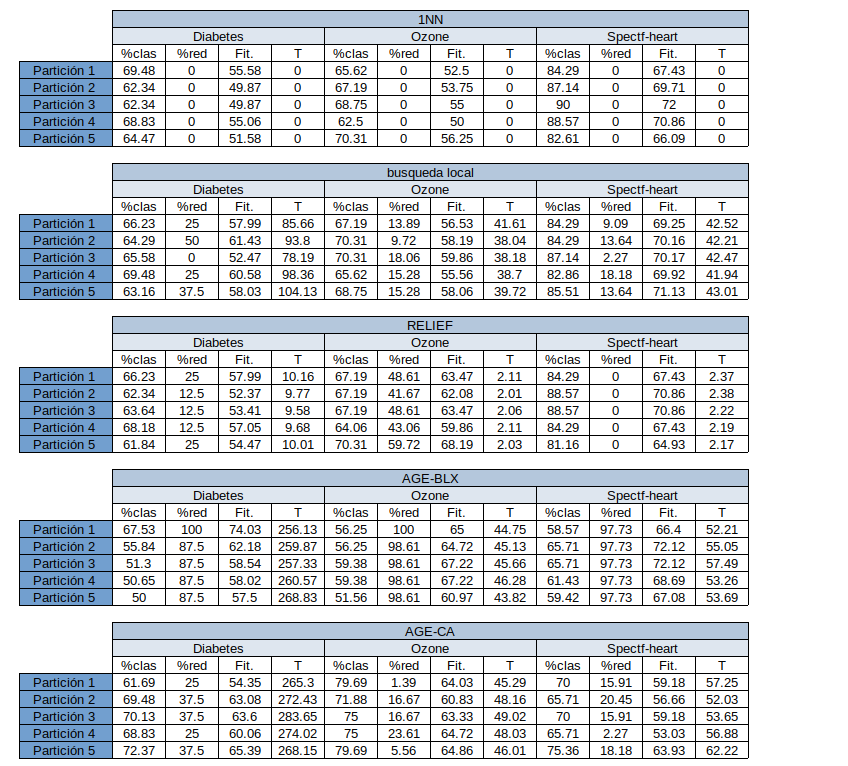
\includegraphics[width=\textwidth]{tables1.png}
  \caption{Tablas de prácticas anteriores}
  \label{fig:imagen}
\end{figure}

\begin{figure}[htbp]
  \centering
  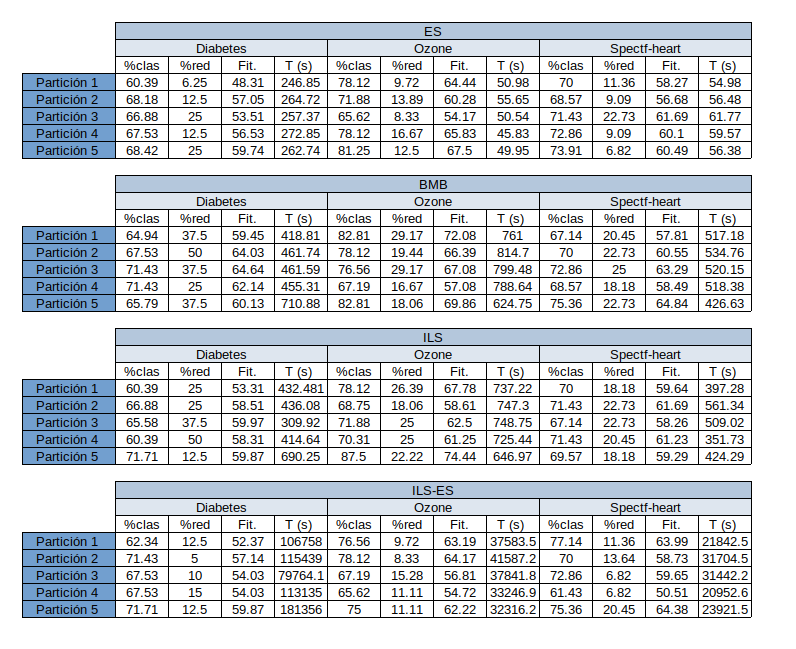
\includegraphics[width=\textwidth]{tables2.png}
  \caption{Tablas de esta práctica}
  \label{fig:imagen}
\end{figure}


\begin{figure}[htbp]
  \centering
  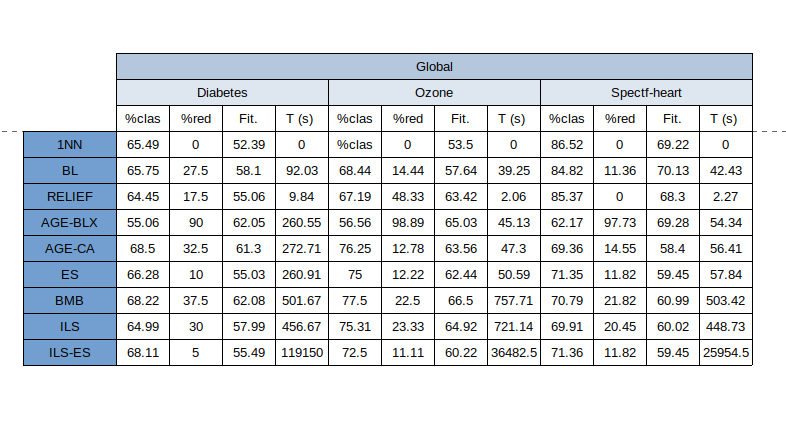
\includegraphics[width=\textwidth]{tables3.png}
  \caption{Tabla de resultados globales}
  \label{fig:imagen}
\end{figure}


\pagebreak
\section{Análisis de resultados}
A continuación se presenta un análisis de las tablas anteiores. 
\subsection{representación gráfica de las soluciones}
\subsubsection{Porcentaje de clasificación}
\begin{tikzpicture}  
\begin{axis}  
[  
  width=18cm,
  ybar, % ybar command displays the graph in horizontal form, while the xbar command displays the graph in vertical form.  
  enlargelimits=0.20,% these limits are used to shrink or expand the graph. The lesser the limit, the higher the graph will expand or grow. The greater the limit, the more graph will shrink.   
  legend style={at={(0.4,-0.25)}, % these are the measures of the bottom row containing surplus (wheat, Tea, rice), where -0.25 is the gap between the bottom row and the graph.   
  anchor=north,legend columns=-1},     
  % here, north is the position of the bottom legend row. You can specify the east, west, or south direction to shift the location.   
  ylabel={\#Porcentaje clasificación}, % there should be no line gap between the rows here. Otherwise, latex will show an error.  
  symbolic x coords={1NN, BL, RELIEF, AGE-BLX, AGE-CA, ES, BMB, ILS, ILS-ES},  
  xtick=data,  
  nodes near coords,  
  nodes near coords align={vertical},  
]  
\addplot coordinates {(1NN, 65.49) (BL, 65.75) (RELIEF, 64.45) (AGE-BLX, 55.06) (AGE-CA, 68.5) (ES, 66.28) (BMB, 68.22) (ILS, 64.99) (ILS-ES, 68.11)};
\addplot coordinates {(1NN, 68.75) (BL, 68.44) (RELIEF, 67.19) (AGE-BLX, 56.56) (AGE-CA, 76.25) (ES, 75) (BMB, 77.5) (ILS, 75.31) (ILS-ES, 72.5)};
\addplot coordinates {(1NN, 86.52) (BL, 84.82) (RELIEF, 85.37) (AGE-BLX, 62.17) (AGE-CA, 69.36) (ES, 71.35) (BMB, 70.79) (ILS, 69.91) (ILS-ES, 71.36)};
\legend{Diabetes, Ozone, Spectf-heart}  
  
\end{axis}  
\end{tikzpicture} 

\pagebreak

\textbf{Análisis de la gráfica}\\
En este gráfico se puede ver como el algoritmo con mayor porcentaje de clasificación es sorprendentemente, 1NN, el algoritmo base. Sin embargo, esto solo pasa con la base de datos Spectf-heart. Con el resto de bases de datos, la tendencia parece ser justo la contraria y el porcentaje de clasificación aumenta incrementalmente con los algoritmos de cada práctica, de forma que los algoritmos basados en trayectorias son los mejores en este aspecto, seguidos de los genéticos.
\pagebreak

\subsubsection{Porcentaje de reducción}
\begin{tikzpicture}  
\begin{axis}  
[  
  width=18cm,
  ybar, % ybar command displays the graph in horizontal form, while the xbar command displays the graph in vertical form.  
  enlargelimits=0.20,% these limits are used to shrink or expand the graph. The lesser the limit, the higher the graph will expand or grow. The greater the limit, the more graph will shrink.   
  legend style={at={(0.4,-0.25)}, % these are the measures of the bottom row containing surplus (wheat, Tea, rice), where -0.25 is the gap between the bottom row and the graph.   
  anchor=north,legend columns=-1},     
  % here, north is the position of the bottom legend row. You can specify the east, west, or south direction to shift the location.   
  ylabel={\#Porcentaje reducción}, % there should be no line gap between the rows here. Otherwise, latex will show an error.  
  symbolic x coords={1NN, BL, RELIEF, AGE-BLX, AGE-CA, ES, BMB, ILS, ILS-ES},  
  xtick=data,  
  nodes near coords,  
  nodes near coords align={vertical},  
]  
\addplot coordinates {(1NN, 0) (BL, 27.5) (RELIEF, 17.5) (AGE-BLX, 90) (AGE-CA, 32.5) (ES, 10) (BMB, 37.5) (ILS, 30) (ILS-ES, 5)};
\addplot coordinates {(1NN, 0) (BL, 14.44) (RELIEF, 48.33) (AGE-BLX, 98.89) (AGE-CA, 12.78) (ES, 12.22) (BMB, 22.5) (ILS, 23.33) (ILS-ES, 11.11)};
\addplot coordinates {(1NN, 0) (BL, 11.36) (RELIEF, 0) (AGE-BLX, 97.73) (AGE-CA, 14.55) (ES, 11.82) (BMB, 21.82) (ILS, 20.45) (ILS-ES, 11.82)};

\legend{Diabetes, Ozone, Spectf-heart}  
  
\end{axis}  
\end{tikzpicture}  

\pagebreak
\textbf{Análisis de la gráfica}\\
El algoritmo con mayor porcentaje de reducción es el Algoritmo Genético Estacionario con el cruce BLX, que es precisamente el algoritmo con menor porcentaje de clasificación. Esto hace pensar que quizás había un bias en la implementación del algoritmo que de alguna forma premiase la reducción muy por encima de la clasificación. \\
\newline
Si se ignora la anomalía del algoritmo AGE-BLX se puede ver también como la base de datos de Diabetes tiende a ser mucho más fácil de reducir mientras que la base de datos de Spectf-heart es la más fácil de reducir. La Búsqueda Multiarranque Básica parece la más apropiada para conseguir buenos resultados de reducción. 

\pagebreak

\begin{tikzpicture}  
\begin{axis}  
[  
  width=18cm,
  ybar, % ybar command displays the graph in horizontal form, while the xbar command displays the graph in vertical form.  
  enlargelimits=0.20,% these limits are used to shrink or expand the graph. The lesser the limit, the higher the graph will expand or grow. The greater the limit, the more graph will shrink.   
  legend style={at={(0.4,-0.25)}, % these are the measures of the bottom row containing surplus (wheat, Tea, rice), where -0.25 is the gap between the bottom row and the graph.   
  anchor=north,legend columns=-1},     
  % here, north is the position of the bottom legend row. You can specify the east, west, or south direction to shift the location.   
  ylabel={\#Fitness}, % there should be no line gap between the rows here. Otherwise, latex will show an error.  
  symbolic x coords={1NN, BL, RELIEF, AGE-BLX, AGE-CA, ES, BMB, ILS, ILS-ES},  
  xtick=data,  
  nodes near coords,  
  nodes near coords align={vertical},  
]  
\addplot coordinates {(1NN, 52.39) (BL, 58.1) (RELIEF, 55.06) (AGE-BLX, 62.05) (AGE-CA, 61.3) (ES, 55.03) (BMB, 62.08) (ILS, 57.99) (ILS-ES, 55.49)};
\addplot coordinates {(1NN, 53.5) (BL, 57.64) (RELIEF, 63.42) (AGE-BLX, 65.03) (AGE-CA, 63.56) (ES, 62.44) (BMB, 66.5) (ILS, 64.92) (ILS-ES, 60.22)};
\addplot coordinates {(1NN, 69.22) (BL, 70.13) (RELIEF, 68.3) (AGE-BLX, 69.28) (AGE-CA, 58.4) (ES, 59.45) (BMB, 60.99) (ILS, 60.02) (ILS-ES, 59.45)};

\legend{Diabetes, Ozone, Spectf-heart}  
  
\end{axis}  
\end{tikzpicture}  

\pagebreak
\textbf{Análisis de la gráfica}\\
Esta gráfica incluye una combinación de las dos anteriores. Por este motivo se puede ver que AGE-BLX se integra con el resto de los resultados sin resaltar como excepción. \\
\newline 
Otra cosa que se puede apreciar es que las metaheurísticas basadas en trayectorias funcionan peor para la base de datos Spect-heart mientras que para la base de datos de Ozone presentan los mejores resultados. \\
\newline 
Si ignoramos el empeoramiento de los resultados para la base de datos Spectf-heart, el valor del fitness tiende a mejorar con cada práctica. 
\pagebreak

\begin{tikzpicture}  
\begin{axis}  
[  
  width=18cm,
  ybar, % ybar command displays the graph in horizontal form, while the xbar command displays the graph in vertical form.  
  enlargelimits=0.20,% these limits are used to shrink or expand the graph. The lesser the limit, the higher the graph will expand or grow. The greater the limit, the more graph will shrink.   
  legend style={at={(0.4,-0.25)}, % these are the measures of the bottom row containing surplus (wheat, Tea, rice), where -0.25 is the gap between the bottom row and the graph.   
  anchor=north,legend columns=-1},     
  % here, north is the position of the bottom legend row. You can specify the east, west, or south direction to shift the location.   
  ylabel={\#Tiempo}, % there should be no line gap between the rows here. Otherwise, latex will show an error.  
  symbolic x coords={1NN, BL, RELIEF, AGE-BLX, AGE-CA, ES, BMB, ILS, ILS-ES},  
  xtick=data,  
  nodes near coords,  
  nodes near coords align={vertical},  
]  
\addplot coordinates {(1NN, 0) (BL, 92.03) (RELIEF, 9.84) (AGE-BLX, 260.55) (AGE-CA, 272.71) (ES, 260.91) (BMB, 501.67) (ILS, 456.67) (ILS-ES, 1294.68401282191)};
\addplot coordinates {(1NN, 0) (BL, 39.25) (RELIEF, 2.06) (AGE-BLX, 45.13) (AGE-CA, 47.3) (ES, 50.59) (BMB, 757.71) (ILS, 721.14) (ILS-ES, 929.489747770701)};
\addplot coordinates {(1NN, 0) (BL, 42.43) (RELIEF, 2.27) (AGE-BLX, 54.34) (AGE-CA, 56.41) (ES, 57.84) (BMB, 503.42) (ILS, 448.73) (ILS-ES, 611.702644355409)};


\legend{Diabetes, Ozone, Spectf-heart}  
  
\end{axis}  
\end{tikzpicture}  

\pagebreak
\textbf{Análisis de la gráfica}\\
En la gráfica anterior se podía apreciar como los resultados mejoraban con cada práctica. Vemos que el tiempo de ejecución también mejora con cada práctica. Esto puede indicar que la mejora en el fitness está estrechamente relacionada con la cantidadd de tiempo que un algoritmo está ejecutándose, y los algoritmos basados en trayectorias no son mejores por si mismos sino más bien porque permiten ejecutar el algoritmo durante más tiempo, lo que a su vez hace que mejore el valor de la evaluación. \\
\newline
Una excepción a esto que se acaba de mencionar el el algoritmo ILS-ES. Algo que se puede apreciar muy bien visiblemente es que ILS-ES es mucho más lento que el resto de metaheurísticas a pesar de que los resultados dejan mucho que desear. 
\pagebreak
\subsection{análisis comparativo de las soluciones obtenidas}
A grandes rasgos en la gráfica de barras del tiempo requerido se puede ver como por lo general, los algoritmos de cada práctica necesitan más tiempo de ejecución que los de la anterior. Eso es algo que no ha sido un inconveniente para realizar esta práctica gracias a la ejecución modular. 
\subsubsection{1-NN}
Este es el algoritmo base que hay que mejorar así que como era de esperar tiene las tasas de clasificación y reducción más bajas, aún así el tiempo de ejecución es casi despreciable. El porcentaje de clasificación es soprendentemente mejor para Spect-heart.

\subsubsection{Busqueda Local}
El porcentaje de clasificación tanto como el de reducción son los mejores en la mayor parte de los casos, descartando en Ozone, donde la reducción de RELIEF es mejor. 

\subsubsection{RELIEF}
Los resultados tienden a ser mejores que 1-NN pero inferiores a BL. En algunos casos puede presentar los mejores resultados, como en el porcentaje de clasificación de Ozone o el porcentaje de reducción de Spect-heart. El tiempo requerido también es varios ordenes de magnitud inferior al requerido por BL. 

\subsubsection{AGE-BLX}
El porcentaje de reducción, así como el porcentaje de clasificación son notablemente mejores que los de los algoritmos de la práctica anterior. Sin embargo, el tiempo en los algoritmos genéticos también avanza mucho. \\
\newline
Curiosamente, el cruce BLX produce los porcentajes de clasificación más bajos y los porcentajes de reducción más altos. 
\subsubsection{AGE-CA}
El porcentaje de reducción es preocupantemente bajo en comparación con el algoritmo que utiliza BLX. Cabe preguntarse si eso es debido a algún error en la implementación del operador de cruce. El tiempo de ejecución también es muy alto en comparación a los algoritmos anteriores. 

\subsubsection{Enfriamiento Simulado}
Vamos a comprarlo con la BL ya que ambos son algoritmos que se podrían considerar como algoritmos de exploración. Se puede comprobar que el ES tiende a reducir menos que la BL, pero su clasificación suele ser mayor. Como resultado, la función de fitness da valores ligeramente peores a pesar de que su tiempo de ejecución es superior al de la búsqueda local.

\subsubsection{Búsqueda Multiarranque Básica}
De manera intuitiva se podía ver que los resultados serían mejores que los de la búsqueda local, ya que consiste en ejecutar la búsqueda local en diferentes sitios y quedarnos con el mejor resultado. \\
La experimentación no nos decepciona y se puede comprobar como efectivamente se consigen valores muy superiores a los de la búsqueda local, tanto en clasificación como reducción. La unica excepción es en Spectf-heart, donde BL consigue el mejor valor de fitness de toda la práctica. 

\subsubsection{Iterative Local Search}
Presenta una tasa de clasificación ligeramente inferior al Enfriamiento Simulado pero un porcentaje superior en varios valores de magnitud, lo que hace que su nivel de fitness tienda a ser superior. 

\subsubsection{ILS-ES}
Como era de esperar los resultados de la hibridación ILS-ES son una mezcla de los resultados de ILS y ES. Por ejemplo esto se puede ver si comparamos el porcentaje de reducción de ILS e ILS-ES. El de la hibridación con Enfriamiento Simulado es mucho menor, de la misma forma que veíamos que el porcentaje de reducción en ES era mucho menor que el de BL. \\
\newline
Los resultados de este algoritmo definitivamente no son los mejores de esta práctica y solo mejoran ligeramente en comparación con los de nuestro algoritmo de referencia 1NN. Además es el más lento de ejecutar con diferencia. 

\subsection{Conclusión}
Si hubiera que decidir cual es el algoritmo superior para el problema de Aprendizaje de Pesos en Carácterísticas, se podría afirmar que BMB es el que mejores resultados da. Su nivel de fitness tiende a ser el mejor, añadiendo una sobrecarga muy ligera en tiempo y una implementación simple e intuitiva. \\
\newline 
Aún así, una lección que podemos sacar de las prácticas de Metaheurísticas es que no hay una metaheuristica que sea superior a las demás en general. Todo depende del problema en el que se esté ejecutando, ya que del resultado dependen muchos factores como la cantidad de elementos que tenemos para entrenar nuestro modelo, la cantidad de características de cada elemento o la importancia del valor de fitness respecto a la importancia de conseguir unos resultados rápidos. Todos estos y muchos más son factores a tener en cuenta a la hora de elegir una metaheuristica para un problema. No hay una metaheurística universal superior a las demás y solo a base de experimentación y análisis podemos encontrar la más adecuada para un problema. 
\pagebreak
\section{Referencias bibliográficas}
Artificial Intelligence: A Modern Approach" (Inteligencia Artificial: Un Enfoque Moderno) de Stuart Russell y Peter Norvig \\
\newline
https://www.latex-project.org/ : El sitio web oficial de LaTeX ofrece una gran cantidad de información, incluyendo tutoriales, guías y documentación completa sobre LaTeX
\end{document}